\documentclass[10pt]{beamer}

% Modern theme configuration
\usetheme{Madrid}
\usecolortheme{orchid} % Cleaner purple/blue look
\usefonttheme{professionalfonts}

% Custom Colors
\definecolor{DeepNavy}{RGB}{0, 33, 71}
\definecolor{EmeraldGreen}{RGB}{0, 155, 119}
\setbeamercolor{palette primary}{bg=DeepNavy, fg=white}
\setbeamercolor{palette secondary}{bg=DeepNavy!80, fg=white}
\setbeamercolor{palette tertiary}{bg=DeepNavy!60, fg=white}
\setbeamercolor{titlelike}{parent=palette primary}
\setbeamercolor{structure}{fg=DeepNavy}

% Packages
\usepackage[utf8]{inputenc}
\usepackage[T1]{fontenc}
\usepackage{amsmath,amssymb}
\usepackage{booktabs}
\usepackage{tikz}
\usetikzlibrary{shapes.geometric, arrows.meta, positioning, calc}
\usepackage{graphicx}

% Metadata
\title[Emotion Detection with TDA]{Emotion Detection from Social Media Posts \\ with Ambiguity Detection}
\subtitle{Using Topological Data Analysis (TDA)}
\author[Arjeet Singh]{Arjeet Singh}
\institute[IIIT-S]{Indian Institute of Information Technology Senapati, Manipur}
\date{April 2026}

\begin{document}

% Title Page
\begin{frame}[plain]
    \titlepage
\end{frame}

% Slide 1
\textbf{Introduction}
\begin{itemize}
    \item Emotion detection is critical for understanding social media sentiment.
    \item Traditional models force every input into a fixed class, even when ambiguous.
\end{itemize}

\vspace{0.3cm}
\textbf{Objective}
\begin{itemize}
    \item Develop a system that can explicitly flag \textbf{ambiguous} inputs.
    \item Use Topological Data Analysis (TDA) to quantify semantic uncertainty.
\end{itemize}

\vspace{0.3cm}
\textbf{Contribution}
\begin{itemize}
    \item Integration of TDA persistence landscapes with BERT and XGBoost.
    \item Novel ambiguity detection rules based on geometric "loop count" (H1).
    \item Robustness against "confident-but-wrong" failure modes in NLP.
\end{itemize}


% Slide 2
\textbf{Existing Work}
\begin{itemize}
    \item BERT and Sentence-BERT models are state-of-the-art for emotion classification.
    \item Datasets like GoEmotions provide fine-grained labels (28 categories).
\end{itemize}

\vspace{0.2cm}
\textbf{Problems with Existing Work}
\begin{itemize}
    \item \textbf{Forced Choice:} Models must pick a class even for nonsensical or mixed-emotion text.
    \item \textbf{Overconfidence:} Neural networks are often overconfident on samples they haven't seen.
\end{itemize}

\vspace{0.2cm}
\textbf{Why This Project is Needed}
\begin{itemize}
    \item Real-world data is messy; sarcasm and semantic overlaps create genuine ambiguity.
    \item Identifying "I don't know" is as important as a correct classification.
\end{itemize}

\vspace{0.2cm}
\textbf{The Solution}
\begin{itemize}
    \item TDA analyzes the \textbf{geometry} of the training neighborhood.
    \item Complex shapes (loops) in the neighborhood signal high uncertainty.
\end{itemize}


% Slide 3
\begin{frame}{Proposed System / Architecture}
    \begin{columns}
        \begin{column}{0.5\textwidth}
            \textbf{System Steps}
            \begin{enumerate}
                \item \textbf{Input:} Raw Reddit text.
                \item \textbf{Embedding:} Compute 768-dim BERT vector.
                \item \textbf{Topology:} Find 24 neighbours; compute H1 loops.
                \item \textbf{Fusion:} Merge Embedding, TF-IDF, and TDA.
                \item \textbf{XGBoost:} Predict class probabilities.
                \item \textbf{Detection:} Apply Ambiguity Rules.
            \end{enumerate}
            \vspace{0.2cm}
            \textbf{Tools:} Python, Giotto-TDA, XGBoost, Transformers.
        \end{column}
        \begin{column}{0.5\textwidth}
            \centering
            \resizebox{!}{0.7\textheight}{
            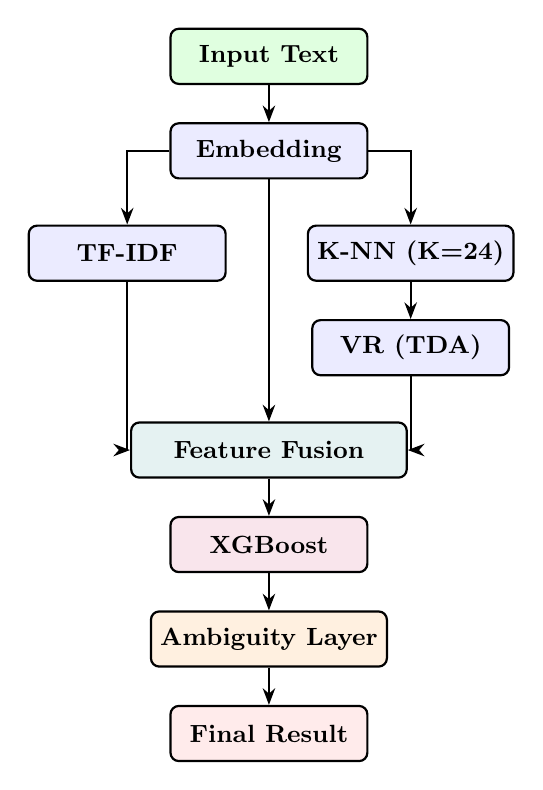
\begin{tikzpicture}[
              font=\small,
              box/.style={draw, rectangle, rounded corners=3pt, thick, align=center, minimum width=2.5cm, minimum height=0.7cm, fill=blue!8},
              widebox/.style={draw, rectangle, rounded corners=3pt, thick, align=center, minimum width=3.5cm, minimum height=0.7cm, fill=teal!10},
              arr/.style={-{Stealth[length=6pt]}, thick}
            ]
              \node[box, fill=green!12] (input) at (0,0) {\textbf{Input Text}};
              \node[box] (embed) at (0,-1.2) {\textbf{Embedding}};
              \node[box] (tfidf) at (-1.8,-2.5) {\textbf{TF-IDF}};
              \node[box] (knn)   at (1.8,-2.5) {\textbf{K-NN (K=24)}};
              \node[box] (vr)    at (1.8,-3.7) {\textbf{VR (TDA)}};
              \node[widebox] (fusion) at (0,-5.0) {\textbf{Feature Fusion}};
              \node[box, fill=purple!10] (xgb) at (0,-6.2) {\textbf{XGBoost}};
              \node[box, fill=orange!12] (ambig) at (0,-7.4) {\textbf{Ambiguity Layer}};
              \node[box, fill=red!8] (output) at (0,-8.6) {\textbf{Final Result}};

              \draw[arr] (input) -- (embed);
              \draw[arr] (embed.west) -| (tfidf.north);
              \draw[arr] (embed.east) -| (knn.north);
              \draw[arr] (embed.south) -- (fusion.north);
              \draw[arr] (knn) -- (vr);
              \draw[arr] (tfidf.south) |- (fusion.west);
              \draw[arr] (vr.south)    |- (fusion.east);
              \draw[arr] (fusion) -- (xgb);
              \draw[arr] (xgb) -- (ambig);
              \draw[arr] (ambig) -- (output);
            \end{tikzpicture}
            }
        \end{column}
    \end{columns}
\end{frame}


% Slide 4
\begin{frame}[fragile]{Result and Analysis}
    \textbf{Experimental Setup}
    \begin{itemize}
        \item \textbf{Dataset:} GoEmotions (43,410 training samples, 5,427 test).
        \item \textbf{Evaluation:} Accuracy and Macro F1-score for 3-class mapping.
    \end{itemize}

    \vspace{0.2cm}
    \textbf{Quantitative Results}
    \begin{table}
        \centering
        \small
        \begin{tabular}{lccc}
            \toprule
            \textbf{Model Version} & \textbf{Accuracy} & \textbf{Macro F1} & \textbf{Ambiguity Flag} \\
            \midrule
            Embeddings only        & 0.57 & 0.52 & No \\
            Embeddings + TF-IDF    & 0.58 & 0.54 & No \\
            \textbf{Proposed (TDA)} & \textbf{0.59} & \textbf{0.56} & \textbf{Yes} \\
            \bottomrule
        \end{tabular}
        \caption{Performance Comparison Table}
    \end{table}

    \vspace{0.1cm}
    \textbf{Key Finding:}
    TDA features provide independent signals that identify cases where the classifier is uncertain due to neighborhood geometry, even when class probabilities are similar.
\end{frame}


% Slide 5
\begin{frame}{Conclusion}
    \textbf{Summary of Work}
    \begin{itemize}
        \item Developed a robust emotion detection pipeline for social media text.
        \item Successfully integrated Topological Data Analysis (TDA) to capture geometric uncertainty in semantic neighborhoods.
        \item Implemented a multi-rule ambiguity detection layer that reduces false-positive classifications.
    \end{itemize}

    \vspace{0.4cm}
    \textbf{Future Scope \& Improvements}
    \begin{itemize}
        \item \textbf{Dataset Expansion:} Develop a large-scale, human-annotated dataset specifically for semantic ambiguity.
        \item \textbf{Performance Optimization:} Explore approximate persistence computation to reduce the inference bottleneck.
        \item \textbf{Multilingual Support:} Extend the TDA framework to multilingual embeddings for global sentiment analysis.
    \end{itemize}
\end{frame}


\end{document}
